% !TeX TS-program = 
\documentclass{article}
\usepackage[spanish, es-tabla]{babel}
\usepackage[utf8]{inputenc}

\usepackage[T1]{fontenc}

\usepackage{adjustbox}



%% Sets page size and margins
\usepackage[letterpaper,top=3.5cm,bottom=3.5cm,left=3cm,right=3cm,marginparwidth=0.5cm, headsep = 70pt]{geometry}

%% Useful packages
\usepackage{amsmath}
\usepackage{float}
\usepackage{graphicx}
\usepackage{multirow}
\usepackage{multicol,lipsum}
\usepackage{enumerate , enumitem , mdwlist}

\usepackage{booktabs, makecell}
\usepackage[table,xcdraw]{xcolor}
\usepackage[colorinlistoftodos]{todonotes}
\usepackage[colorlinks=true, allcolors=blue]{hyperref}
\usepackage[hang, small,up,textfont=it,up]{caption} 
\usepackage{fancyhdr}

% estos paquetes hacen árboles, pero cargan 
% xcolor package, so must be bottom
\usepackage{tikz}
\usetikzlibrary{arrows,shapes,positioning,shadows,trees,calc}


\newcommand\fechafinal{27 Julio 2020 }

% subcaptions
% https://tex.stackexchange.com/questions/523462/3-by-2-multi-table
\usepackage{siunitx}
\renewcommand\cellset{\renewcommand\arraystretch{0.84}}
\usepackage[skip=3ex]{subcaption}

%cabecera y pies
\pagestyle{fancy}
\fancyhf{}
\rhead{
\includegraphics[width=0.12\textwidth]{SAMU_e.png}}
\lhead{
UGCC, COVID-19 \\ 
Dr E. Céspedes G. \\
SAMU V Región \\
\fechafinal}
\rfoot{P\'agina \thepage}

% titulo documento
\title{Análisis registros UGCC}
\author{Dr E Céspedes-González}
\date{\fechafinal}


\begin{document}
\maketitle

\tableofcontents

\newpage

\section{Introducción}

Coronavirus19 o COVID19 es el nombre de la pandemia por un virus de la familia de los coronavirus que comienza en China en Diciembre del 2019 en relación a un mercado de animales de Wuhan \cite{wang_novel_2020}. Cuando se alcanzaron los 27 pacientes con neumonia grave 'inexplicable' y ya estaban en curso estudios etiológicos de secuenciación genómica por laboratorios de virología con resultados preliminares que identificaba una nueva especie de coronavirus. El 31 de Diciembre del 2019 la Comisión Municipal de Salud y Sanidad de Wuhan emite un comunicado donde declara 'la transmisión persona a persona de una enfermedad viral que produce neumonia' \cite{oms_oms_2020}.

La enfermedad avanzó rápidamente:  El 13 de Enero 2020 aparece el primer caso en Tailandia, el 16 de Enero en Japón, el 20 de Enero en Estados Unidos. El 30 de Enero la Organización Mundial de la Salud declara emergencia de salud global. El 25 de Febrero aparece el primer caso en Brasil y el 3 de Marzo el primer caso en Chile. Ya para el 1 de Junio 2020 a nivel mundial hay más de 6 millones de infectados, 378.000 muertos y 2.6 millones informados como recuperados \cite{oms_covid-19_2020}.

En la era tecnológica que cursamos cada día hay recursos tecnológicos, de información y de datos más grandes y mejores que antes. Hoy existe la ciencia de datos, el \textit{Big data} y el \textit{Machine Learning}, disciplinas que están haciendo un cambio en las políticas públicas al colaborar en la toma de decisiones. El enfrentamiento de una pandemia o protocolos de circunstancias extraordinarias dista mucho en lo proyectado versus las herramientas realmente disponibles. Pero también hay que ser cauteloso; estas herramientas deben ser utilizadas en manos expertas y sus resultados correctamente interpretados.

Dentro de las distintas estrategias de registro y trazabilidad de los pacientes con Coronavirus19 se implementó la evolución en el sistema que clásicamente se utilizaba para la gestión de unidad de gestión de camas críticas (UGCC).

Actualmente la plataforma de UGCC es una de las fuentes de información con que los distintos servicios de salud cuentan. Esta plataforma  está codificada, es transversal, asequible, en línea y parametrizada. No fue diseñada en principio para fines de la pendemia del Coronavirus19, pero es útil.

El objetivo del siguiente trabajo es describir parte de la información alojada en esta plataforma.




\section{Metodología}
Trabajo descriptivo de ciencia de datos transversal. 

Se buscó y describieron algunas de las bases de datos que existen en el sitio \href{https://ugcc.minsal.cl/}{ugcc.minsal.cl}.

La confidencialidad fue respetada en todo momento al enmascarar identidades por cadenas de texto y caracteres con que es imposible conectar con identidades de pacientes, de esta manera que se analizaron casos enmascarados.
Se utilizó\LaTeX ,  Python 3, y los paquetes para el análisis de datos: pandas, numpy, datetime, matplotlib.


\newpage


\section{Resultados}
Se exploró la web de UGCC, se descargaron algunos set de datos generales para mostrar datos genéricos


\subsection{Las bases de datos disponibles}

Se listan las distintas secciones que se encontraron en la página web de UGCC

\begin{multicols}{2}
\input{./mapa_ugcc.item}
\end{multicols}

\subsection{Derivaciones UGCC}

Se analizó la base de datos de derivaciones que existe en la plataforma web de UGCC. Existen casos Históricos y Exitosa (en los que hubo efectivamente derivación), los y Nulos y Erróneos (en los que el proceso de derivación se detuvo por alguna razón) y los 'Buscando o asignando destino' que están actualmente en curso. 

\input{./textos/texto_descriptorUGCC.txt}




En la Figura \ref{fig: ARBOL derivacionesUGCC} se observa un detalle de las derivaciones desde el año 2010 al 2020, sólo del año 2019 y sólo las de este año. Esta figura permite entender de mejor manera cómo están los datos ingresados en la plataforma UGCC. Cabe destacar que:

\begin{itemize}
	\item Los casos 'Exitosos' están en un proceso administrativo pero cuentan como derivación válida.
	\item Las derivaciones entre el mismo servicio de salud registradas en UGCC no corresponde al total de los casos, ya que no es un hábito asentado de subir datos a la plataforma de los pacientes derivados desde otro hospital de la red.
	\item Los casos Exitosos si bien ya son una derivación, están en algún proceso administrativo.
\end{itemize}
 


\begin{figure}[h]
	\centering
	\begin{subfigure}{.75\textwidth}
		\centering
		\resizebox{.999\textwidth}{!}{
		\begin{tikzpicture}
		[-,thick,
		every node/.style={shape=rectangle,inner sep=3pt,draw,thick, align=center}]
		\footnotesize
		\input{./textos/arbol_derivaciones2010.arbol}   %%%%% arbol leída acá!!!		
		;
		\end{tikzpicture}
		}
		\caption{Derivaciones de pacientes desde el año 2010 hasta la actualidad }
	\end{subfigure}%

	\begin{subfigure}{.75\textwidth}
		\centering
		\resizebox{.999\textwidth}{!}{
		\begin{tikzpicture}
		[-,thick,%
		every node/.style={shape=rectangle,inner sep=3pt,draw,thick, align=center}]
		\footnotesize
		\input{./textos/arbol_derivaciones2019.arbol}   %%%%% arbol leída acá!!!		
		;
		\end{tikzpicture}
		}
		\caption{Derivaciones de pacientes durante el 2019.}
	\end{subfigure}
	\begin{subfigure}{.75\textwidth}
	\centering
	\resizebox{.999\textwidth}{!}{
		\begin{tikzpicture}
		[-,thick,%
		every node/.style={shape=rectangle,inner sep=3pt,draw,thick, align=center}]
		\footnotesize
		\input{./textos/arbol_derivaciones2020.arbol}   %%%%% arbol leída acá!!!		
		;
		\end{tikzpicture}
	}
	\caption{Derivaciones de pacientes durante el 2020.}
	\end{subfigure}
	\caption{Derivación de pacientes en sistema UGCC del SSVQ. Distintos periodos de tiempo}
	\label{fig: ARBOL derivacionesUGCC}
\end{figure}



En la tabla \ref{tab: Derivaciones historicas} se puede observar la cantidad de derivaciones a lo largo de los años según especialidad y otras variables, hay un detalle de la cantidad de derivaciones por hospital y su destino por fecha en la tabla \ref{tab: derivaciones por hospital y destino}. En la Figura \ref{fig: derivacionesUGCC} se puede observar con detalle derivaciones desde hospitales del SSVQ con énfasis en distintos periodos de tiempo. Para mayor compresión de la forma en que se ordenan y analizan los datos y proyección de cifras se puede consultar la Figura \ref{fig: ARBOL derivacionesUGCC}.

\begin{table}[h]
	\begin{subtable}{0.5\textwidth}
		\centering
		\begin{adjustbox}{width=0.95\textwidth}
			\input{./textos/00Derivacionesxespecialidad10a.tab}   %%%%% tabla leída acá!!!		
		\end{adjustbox}
		\caption{Cantidad de derivaciones de pacientes en distintas especialidades desde el año 2010 desde hospitales del SSVQ. Se consideran derivaciones a cama UPC, hacia clínicas y hospitales dentro y fuera del SSVQ}

\vspace{0.7cm}

		\begin{adjustbox}{width=0.7\textwidth}
			\input{./textos/00Derivacionesmensual5a.tab}   %%%%% tabla leída acá!!!
		\end{adjustbox}
	\caption{Cantidad de derivaciones hacia camas UPC por mes desde el año 2015 a la fecha de pacientes adultos. Se incluyen derivaciones a clínicas, hospitales de la red y fuera del SSVQ}
	\end{subtable}%
	\begin{subtable}{0.5\textwidth}
	\centering
	\begin{adjustbox}{width=0.95\textwidth}
		\input{./textos/00Derivacionesxhospital2020.tab}   %%%%% tabla leída acá!!!
	\end{adjustbox}
	\caption{Derivaciones mensuales de pacientes adultos en los tres hospitales de alta complejidad del SSVQ desde el 2017. Se incluyen derivaciones a camas UPC hacia clínicas, hospitales de la red SSVQ y de otros servicios de salud}
\end{subtable}
\caption{Cantidad de derivaciones de pacientes desde el SSVQ según especialidad, distintos periodos de tiempo, según hospital. Se incluyen sólo camas UPC y desde hospital hacia clínicas, hospitales de la red SSVQ y fuera de esta. }
\label{tab: Derivaciones historicas}
\end{table}


\begin{table}[p]
	\begin{adjustbox}{width=0.95\textwidth}
		\input{./textos/00Derivacionesxhospital_detalle.tab}   %%%%% tabla leída acá!!!
	\end{adjustbox}
	\caption{Detalle de derivaciones con distintos destinos para cada centro de alta complejidad del SSVQ desde e año 2017 a la actualidad.} 
	\label{tab: derivaciones por hospital y destino}
\end{table}


\begin{figure}[p]
	\begin{subfigure}{.5\textwidth}
		\centering
		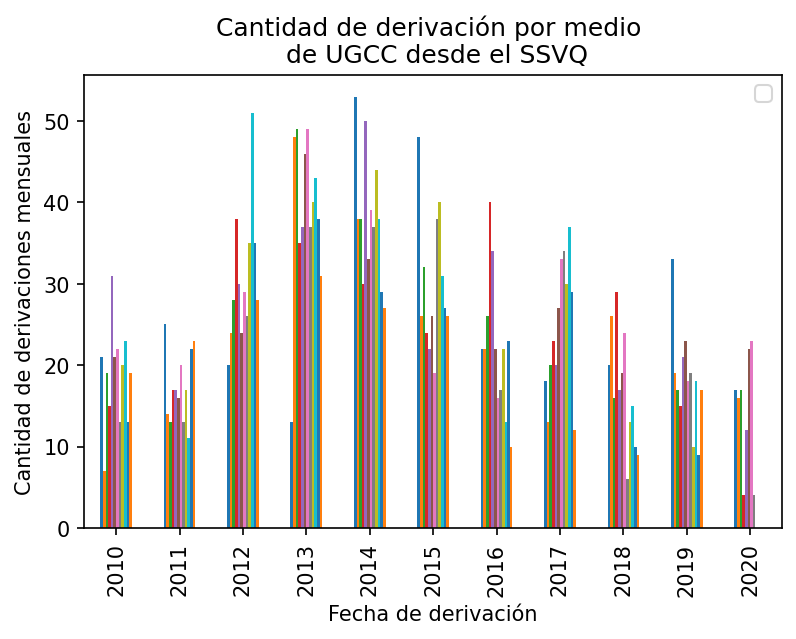
\includegraphics[width=.8\linewidth]{./figuras/Derivaciones10_20.png}
		\caption{Derivaciones de pacientes adultos desde el año 2010 hasta la actualidad. Sólo se muestran derivaciones de pacientes adultos. Se presenta una distribución mensual para valorar la estacionalidad de las derivaciones a lo largo del año.}
	\end{subfigure}%
	\begin{subfigure}{.5\textwidth}
		\centering
		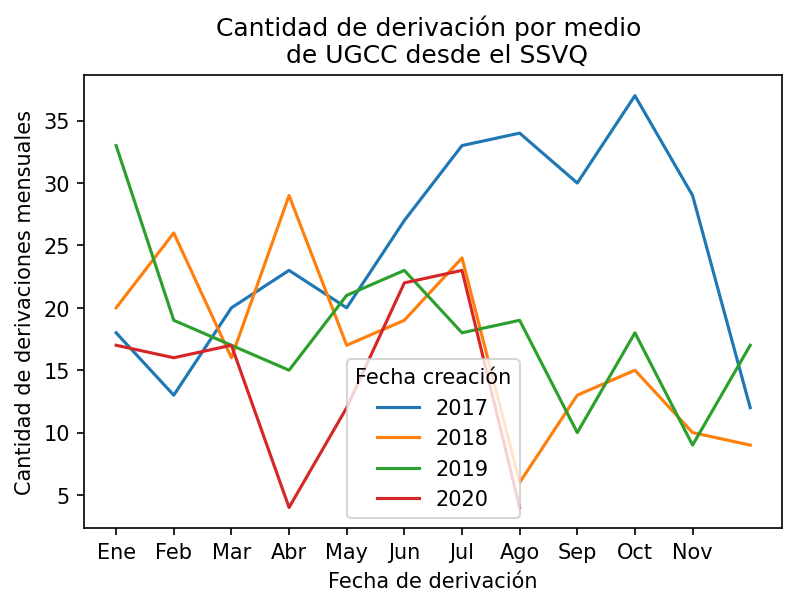
\includegraphics[width=.8\linewidth]{./figuras/Derivaciones17_20.png}
		\caption{Derivaciones de pacientes adultos desde el año 2017. Sólo se muestran derivaciones de pacientes adultos. Se presenta en detalle la distribución mensual para valorar la estacionalidad de las derivaciones a lo largo de los años previos.}
	\end{subfigure}
	\centering
	\begin{subfigure}{.5\textwidth}
		\centering
		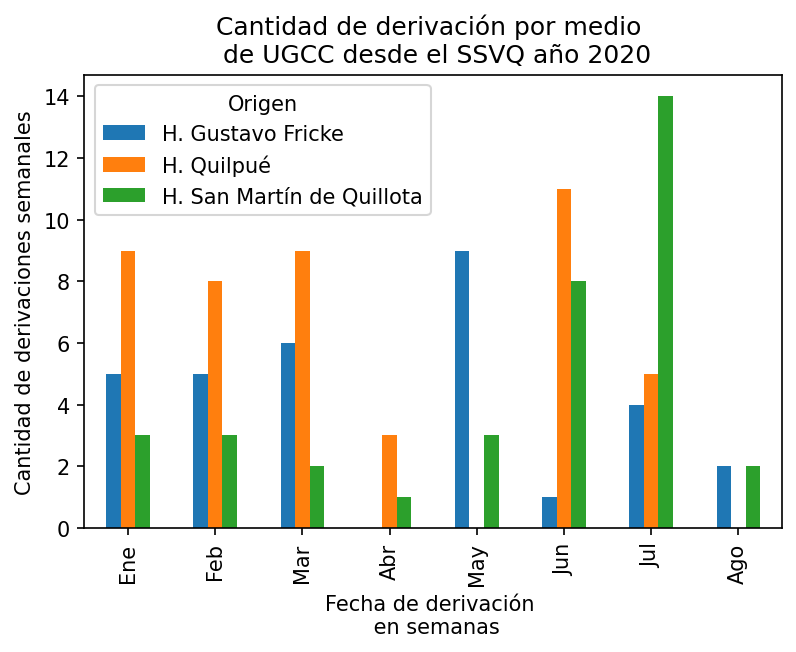
\includegraphics[width=.8\linewidth]{./figuras/Derivaciones2020.png}
		\caption{Derivaciones de pacientes adultos del año 2020 según centro derivador. Se muestra cantidad de derivaciones mensuales.}
	\end{subfigure}
	\caption{Derivación de pacientes en sistema UGCC del SSVQ. Distintos periodos de tiempo}
	\label{fig: derivacionesUGCC}
\end{figure}


La edad de los pacientes sólo se encuentra registrada hasta el año 2013 (1235 registros), la que en los adultos tiene una media de 64 años, edades extremas desde los 15 años hasta los 95 años. El rango intercuartil es desde los 48 a los 74 años.  La media de edad entre los pacientes adultos según el tipo de derivación (Intrapúblico de 62.8 años, Intra SSVQ de 59.7 años y Público a privado 59.3 años) no presentó diferencia significativa con un valor de p menor a 0.05 para la prueba de ANOVA. Se observa en la figura \ref{fig: edadyestadia_derivaciones} un gráfico de cajas y bigotes para este dato.

La estadía de los pacientes tuvo una media de 7 días al ser derivados a un cama crítica, con un rango intercuartil de 4 a 11 días. Según ANOVA no hubo diferencias para las derivaciones hacia centros privados, intra públicos o hacia establecimientos del SSVQ con un valor de p de 0.008. en la figura \ref{fig: edadyestadia_derivaciones} se observa un gráfico de cajas y bigotes para este cálculo.


No hay registro de 

\begin{figure}
	\centering
	\begin{subfigure}{.5\textwidth}
		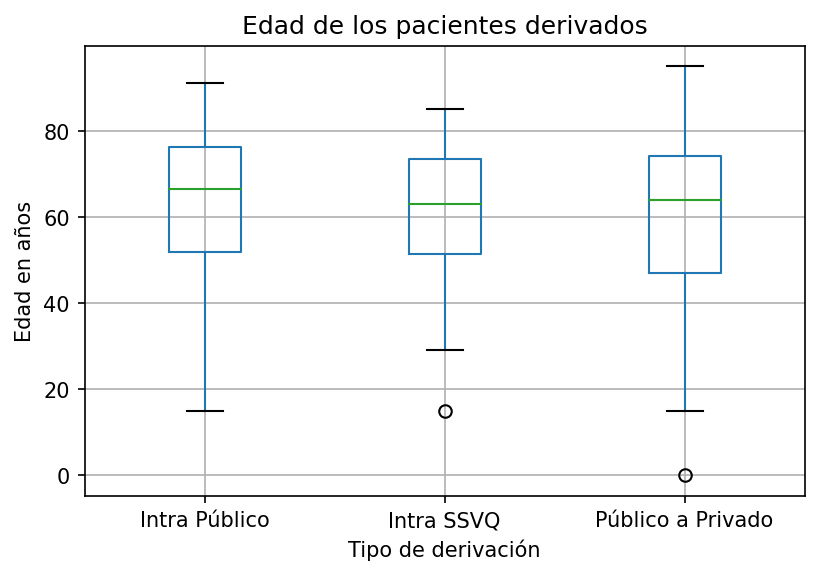
\includegraphics[width=.8\linewidth]{./figuras/Edad_derivacion_historica.png}
	\end{subfigure}%
	\begin{subfigure}{.5\textwidth}
		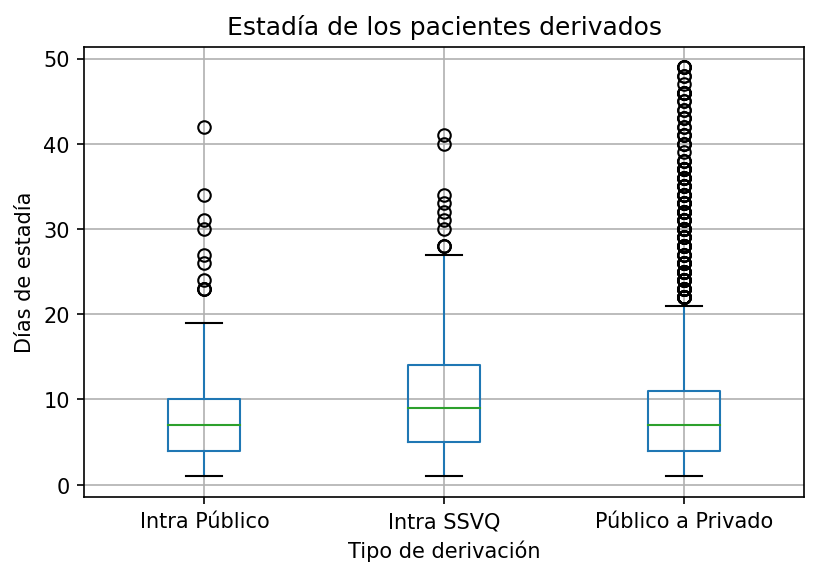
\includegraphics[width=.8\linewidth]{./figuras/Estadia_derivacion_historica.png}
	\end{subfigure}
	\caption{Gráfico de cajas y bigotes para la edad y estadía de pacientes adultos derivados desde el SSVQ entre el 2009 y el 2020 hacia camas críticas según distintas vías de derivación.}
\label{fig: edadyestadia_derivaciones}
\end{figure}



%%%%%%%
%%%%%%%
%%%%%%%
\subsection{Base de datos 'Covid-19'}

El set de datos contiene pacientes atendidos (históricos o están en proceso de atención) en territorio físico del SSVQ además de pacientes con domicilio en territorio del SSVQ (FONASA y no FONASA) con atención en otros servicios de salud. Se debe entender que los datos incluyen pacientes residentes de otros servicios de salud.


\input{./textos/01Descripcion_dataset.txt}

% figura de la incidencia notificaciones
\begin{figure}
	\centering
	\begin{adjustbox}{width=0.6\textwidth}
		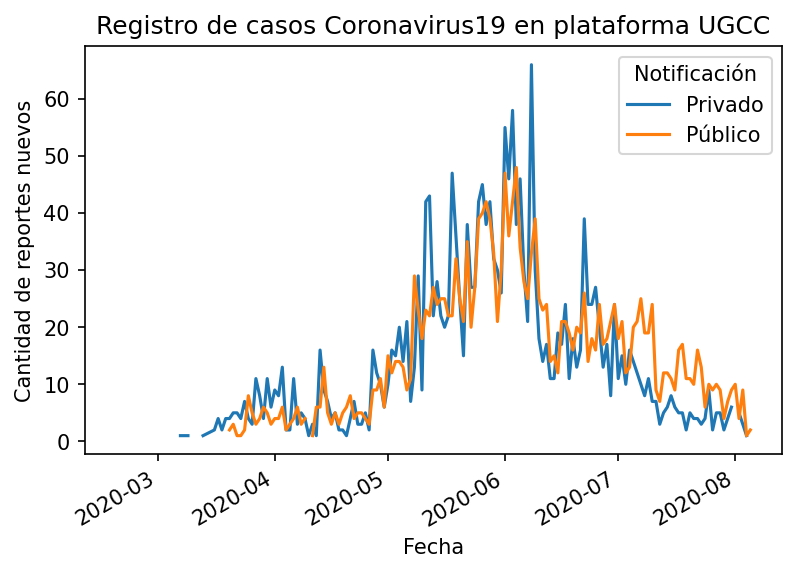
\includegraphics{./figuras/casosnuevosUGCC.png} %%%%% grafo leído acá!!!
	\end{adjustbox}
	\caption{Incidencia de casos nuevos en plataforma UGCC rama Covid-19. Se muestra la cantidad de casos nuevos en el sistema diarios. Se dividen los casos según el tipo público/privado del establecimiento que reporta el caso.}
	\label{fig:movilidad mundial_DS}
\end{figure}


% texto casos duplicados
\input{./textos/02Duplicados.txt}

\medskip

\begin{table}[h]
	\begin{subtable}{0.5\textwidth}
		\centering
		\begin{adjustbox}{width=0.95\textwidth}
			\input{./textos/01TAB_previsionvscentro_total.tab}   %%%%% tabla leída acá!!!
		\end{adjustbox}
		\caption{Todos los casos, incluidos historicos}
	\end{subtable}
	\begin{subtable}{0.5\textwidth}
		\centering
		\begin{adjustbox}{width=0.95\textwidth}
			\input{./textos/01TAB_previsionvscentro_activos.tab}   %%%%% tabla leída acá!!!
		\end{adjustbox}
		\caption{Casos actualmente activos}
	\end{subtable}
	\medskip
	
	\begin{subtable}{0.5\textwidth}
		\centering
		\begin{adjustbox}{width=0.95\textwidth}
			\input{./textos/01TAB_previsionvscentro_activosV.tab}   %%%%% tabla leída acá!!!
		\end{adjustbox}
		\caption{Casos actualmente activos en la V Región}
	\end{subtable}
	\begin{subtable}{0.5\textwidth}
		\centering
		\begin{adjustbox}{width=0.95\textwidth}
				\input{./textos/01TAB_previsionvscentro_activosRM.tab}   %%%%% tabla leída acá!!!
		\end{adjustbox}
		\caption{Casos actualmente activos en la RM}
	\end{subtable}
	\caption{Cantidad de casos FONASA y no-FONASA en distintas situaciones} 
	\label{tab:previsonvsESTABLECIMEITNO}
\end{table}



\newpage
\bibliographystyle{vancouver}
\bibliography{bibliografia,Coronavirus_historia}



\end{document}